\chapter{Część sprzętowa}

Część sprzętowa projektu obejmuje zaprojektowanie oraz zmontowanie PCB - nakładki na płytkę Maximator. Wykorzystany układ FPGA jest zgodny z logiką 2,5 V, dlatego niezbędny był układ kondycjonowania dla wejść, aby zapewnić bezproblemową pracę podczas testowania układów zgodnych z logiką 3,3 V. Dodatkowym celem było zapewnienie interfejsu do sterowania pracą urządzenia.

Wykorzystano pięć przycisków, które służą do:
\begin{itemize}
\item CH+; CH- - zmiana wybranego kanału
\item FASTER; SLOWER - zmiana częstotliwości próbkowania
\item TRIG\_SEL - zmiana sposobu 
\item RESET - sprzętowy reset Maximator'a
\end{itemize}
Dodatkowo znajduje się dioda \textit{TRIG\_STAT} sygnalizująca wyzwolenie zapisu. 


Kondycjonowanie sygnału zostało zrealizowane za pomocą diod transil. Wymagały one osobnego zasilania napięciem 2.5 V, dlatego na płytce został umieszczony stabilizator. Dodatkowo szeregowo do wejścia został umieszczony rezystor o wartości $1 k\Omega$. Ma on za zadanie ograniczać maksymalny prąd, który popłynie podczas włączenia diody. 

Poniżej przedstawiono obliczenia prądu płynącego przez diodę (z pominięciem napięcia na niej) dla napięcia wejściowego równego 3,3 V:
\begin{equation}
I = \frac{3,3\ V - 2,5\ V}{1\ k\Omega} = 0,8\ mA
\label{eq:diode_current}
\end{equation}

\begin{figure}[H]
\begin{center}
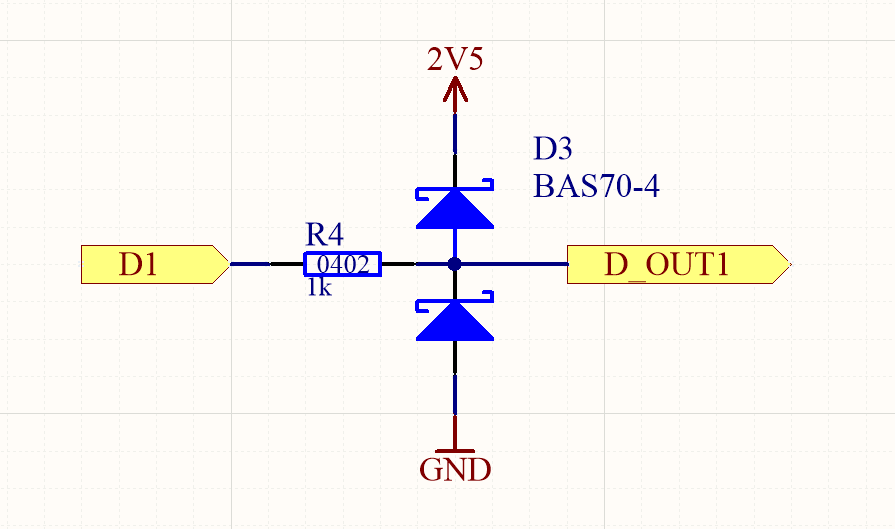
\includegraphics[width=3.5 in]{images/pin_conditioning.png}
\end{center}
\caption{Schemat układu kondycjonowania wejść}
\label{fig:pin_conditioning}
\end{figure}

Jako źródło zasilania diod zastosowano liniowy stabilizator napięcia. Jako źródło wykorzystuje się napięcie 3,3 V dostarczane przez układ \textit{Maximator}. Dodano kondensatory filtrujące w celu wygładzenia napięcia wyjściowego. 

\begin{figure}[H]
\begin{center}
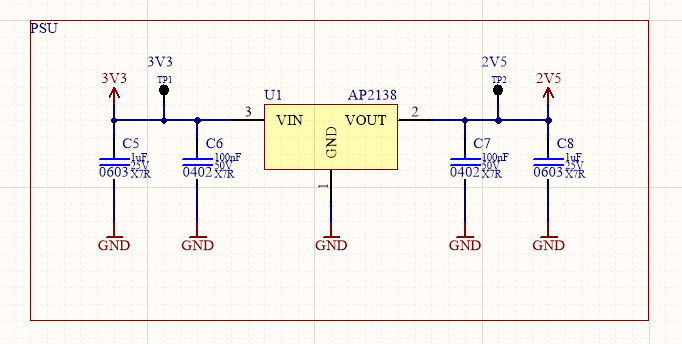
\includegraphics[width=3.5 in]{images/psu.png}
\end{center}
\caption{Schemat stabilizatora napięcia}
\label{fig:psu}
\end{figure}

Poniżej zestawiono pozostałą część schematu ideowego urządzenia.

Przy układach peryferyjnych zastosowano wygładzanie drgań styków za pomocą kondensatorów o pojemności 100 nF. 

\begin{figure}[H]
\begin{center}
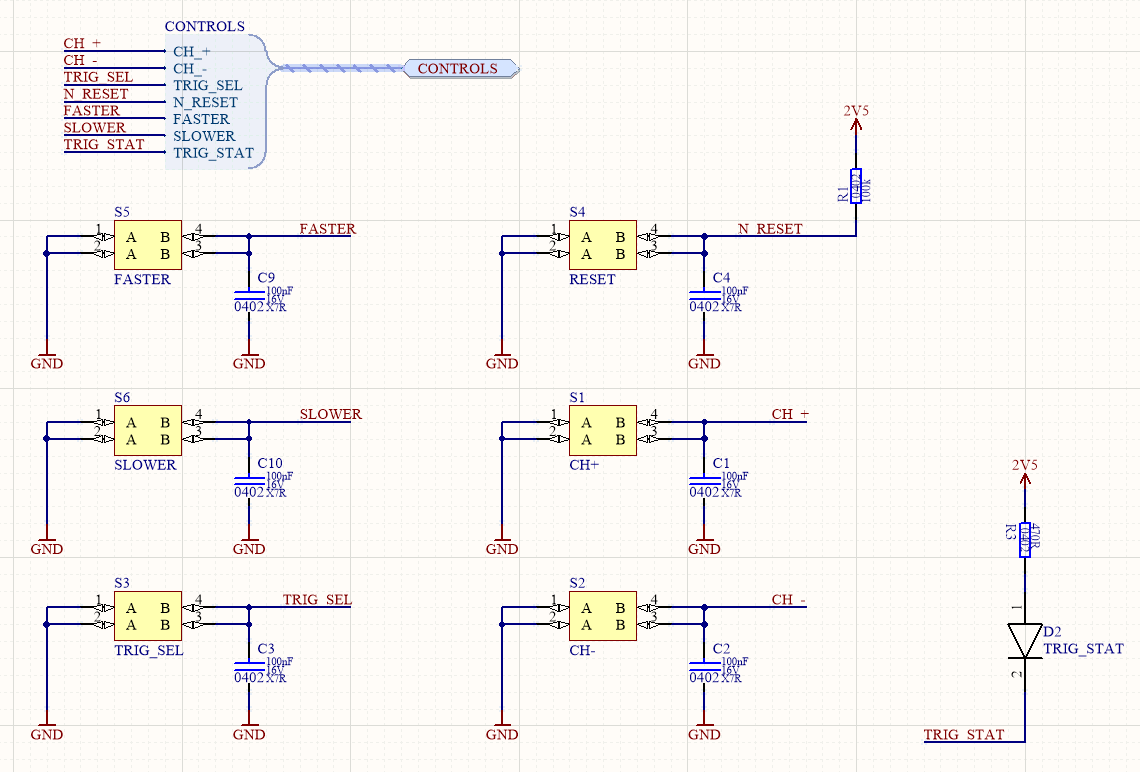
\includegraphics[width=4.5 in]{images/peripherals.png}
\end{center}
\caption{Schemat układów peryferyjnych}
\label{fig:peripherals}
\end{figure}

Schemat połączenia gniazd:

\begin{figure}[H]
\begin{center}
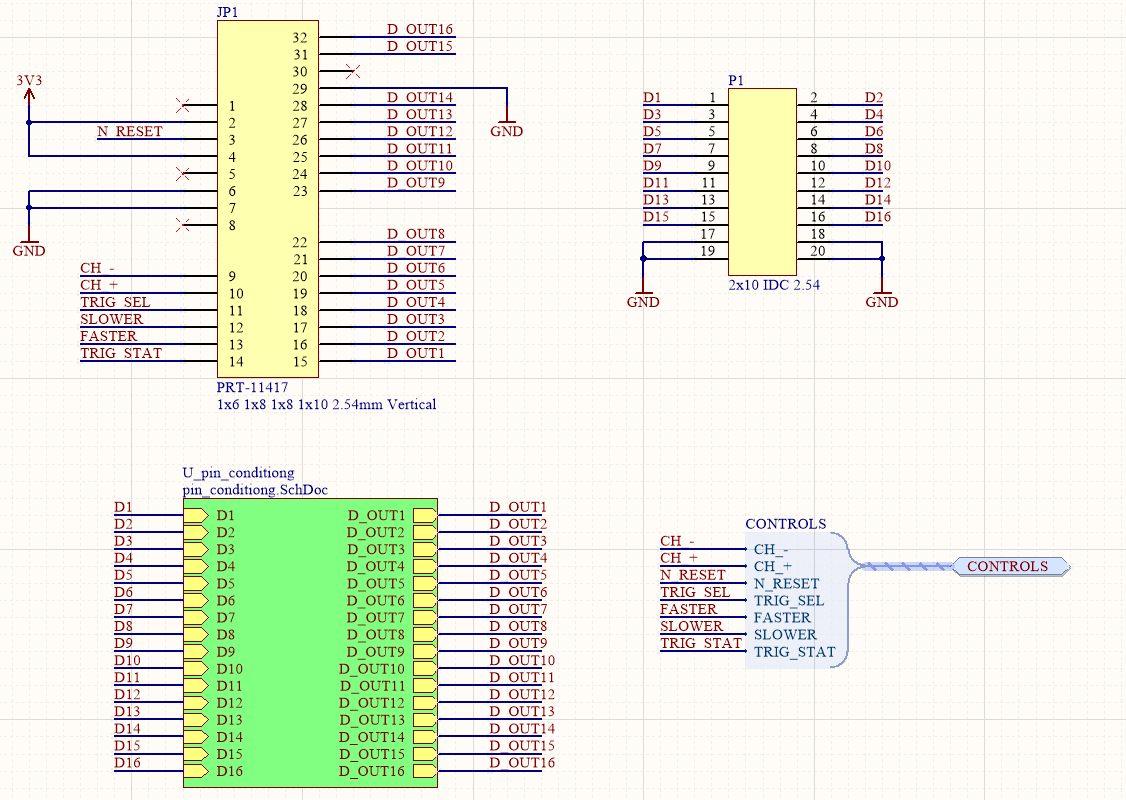
\includegraphics[width=4.5 in]{images/connectors.png}
\end{center}
\caption{Schemat połączeń}
\label{fig:connectors}
\end{figure}

\begin{figure}[H]
\begin{center}
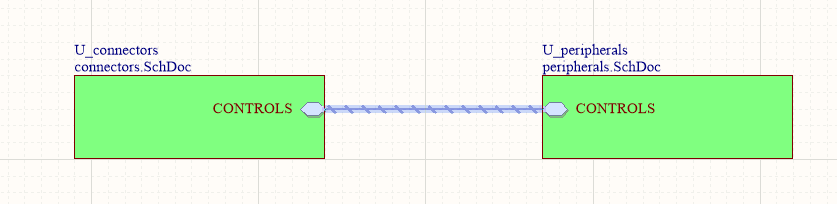
\includegraphics[width=4 in]{images/top.png}
\end{center}
\caption{Schemat połączenia bloków projektowych}
\label{fig:top}
\end{figure}

Wizualizacja 3D płytki:

\begin{figure}[H]
\begin{center}
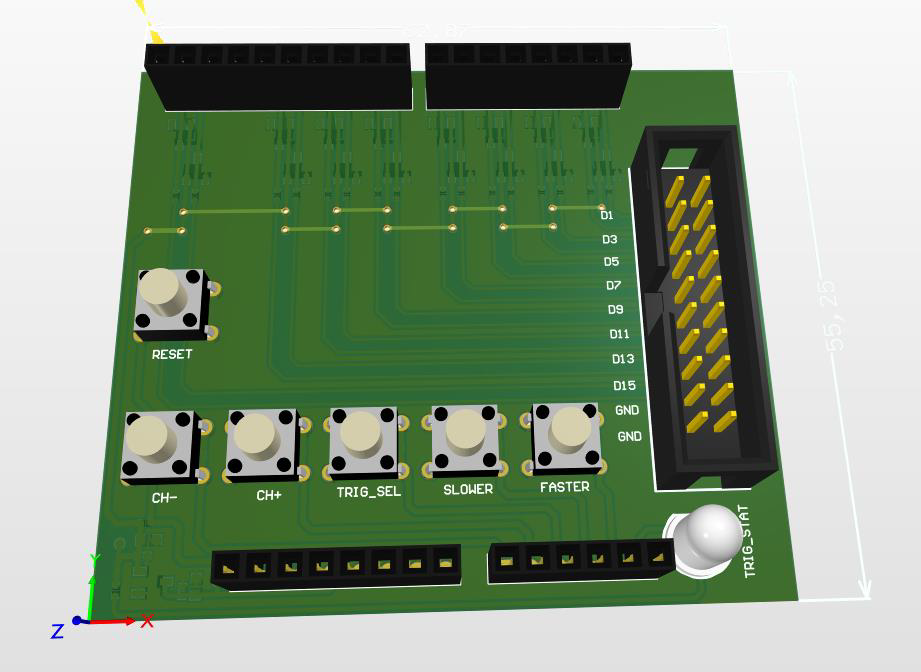
\includegraphics[width=4 in]{images/3D_1.png}
\end{center}
\caption{Widok PCB na warstwę górną}
\label{fig:PCB_top}
\end{figure}

\begin{figure}[H]
\begin{center}
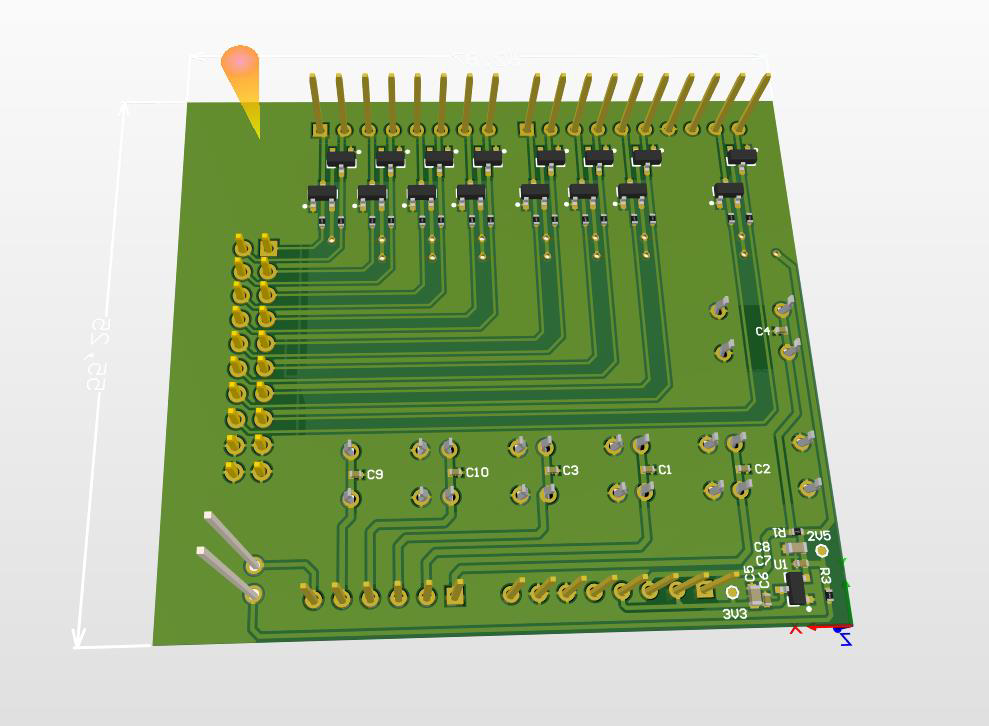
\includegraphics[width=4 in]{images/3D_2.png}
\end{center}
\caption{Widok PCB na warstwę dolną}
\label{fig:PCB_bottom}
\end{figure}

Projekt PCB uwzględniał zachowanie odległości pomiędzy ścieżkami w celu zredukowania zakłóceń podczas transmisji szybkich sygnałów (redukcja wpływu efektu odległościowego - ang. \emph{proximity effect}).